% Sistema de nivel: tanque único con válvula de salida
\documentclass[border=5pt]{standalone}
\usepackage{tikz}
\usetikzlibrary{arrows.meta}
\begin{document}
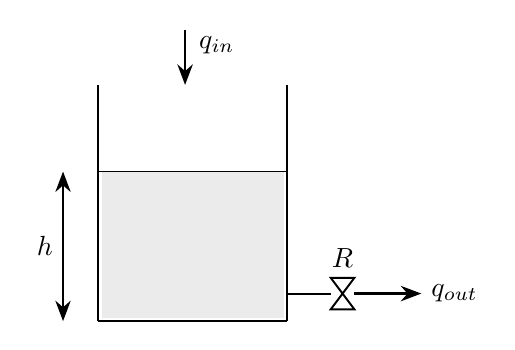
\begin{tikzpicture}[>={Stealth[length=2.6mm]}, line width=0.7pt]
  % caudal de entrada
  \draw[->, line width=1pt] (1.1,3.7) -- (1.1,3.0);
  \node[right] at (1.15,3.5) {$q_{in}$};
  % tanque (U abierto arriba)
  \draw (0,0) -- (0,3) (2.4,0) -- (2.4,3) (0,0) -- (2.4,0);
  % agua
  \fill[black!8] (0.04,0.04) rectangle (2.36,1.9);
  \draw (0,1.9) -- (2.4,1.9);
  % cota h
  \draw[<->] (-0.45,0) -- (-0.45,1.9);
  \node[left] at (-0.45,0.95) {$h$};
  % salida con válvula R (moño)
  \draw (2.4,0.35) -- (2.95,0.35);
  \draw (2.95,0.15) -- (3.25,0.55) -- (2.95,0.55) -- (3.25,0.15) -- cycle;
  \node[above] at (3.1,0.55) {$R$};
  \draw[->, line width=1pt] (3.25,0.35) -- (4.1,0.35);
  \node[right] at (4.1,0.35) {$q_{out}$};
\end{tikzpicture}
\end{document}
